\section{Medición del Entrainment}
\label{sec:method_entrainment}

\begin{figure}
\centering
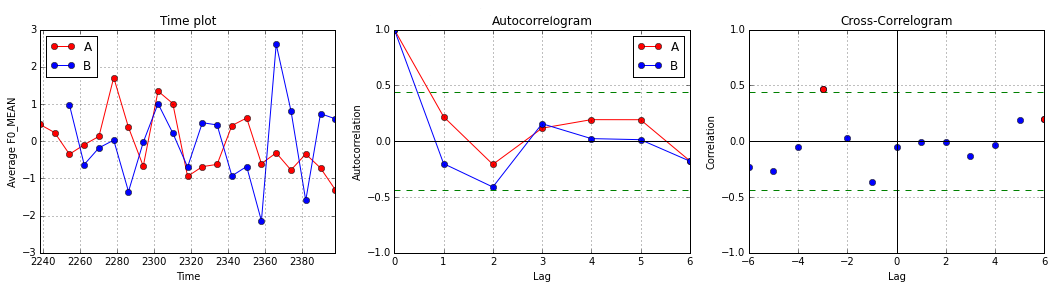
\includegraphics[width=15cm]{images/time_plot_with_cross_correlation.png}
\caption{Time-plot generado por el método TAMA, junto a su autocorrelograma y correlograma cruzado}
\label{fig:time_plot_with_bivariate}
\end{figure}

Considerando todo lo mencionado en la Sección \ref{sec:analisis_bivariado}, procedimos a definir una medida de \entrainment basándonos en el cálculo de la correlación cruzada muestral. Recordemos que, bajo la definición dada en la ecuación \ref{cross_correlation_definition} de $r_{AB}(k)$, al tomar $k \geq 0$ medíamos cuánto influía $B$ sobre los futuros valores de $A$, y viceversa cuando $k \leq 0$. Se tomó la decisión de que este cálculo sólo se realice cuando el desplazamiento resulta en al menos 4 puntos que se solapan; si esto no ocurre, dejamos indefinido el valor en el correlograma cruzado.

Con esto en mente, definimos una primer métrica $\fwentrainment{AB}^{(1)}$ como el valor de $r_{AB}(k)$ con mayor valor absoluto, dado $k \leq 0$. Análogamente lo definimos para $\fwentrainment{BA}^{(1)}$. En \ref{fig:time_plot_with_bivariate} podemos observar en el lag -3 y 6 los valores de \entrainment elegidos del correlograma.

En segundo lugar, definimos una segunda métrica $\fwentrainment{BA}^{(2)}$, como el valor absoluto de la primera, es decir:

\begin{equation}
\fwentrainment{BA}^{(2)} = |\fwentrainment{BA}^{(1)}|
\end{equation}

Por último, cabe mencionar que a diferencia de \cite{KOU2008.2} dónde sólo se hacía un análisis de significancia, nosotros vamos a utilizar esta medida independientemente de si es o no estadísticamente diferente de cero.
